\documentclass[a4paper,twocolumn]{article}%
\usepackage[T1]{fontenc}%
\usepackage[utf8]{inputenc}%
\usepackage{lmodern}%
\usepackage{textcomp}%
\usepackage{lastpage}%
\usepackage{geometry}%
\usepackage{times}%
\usepackage{graphicx}%
%
\geometry{top=19mm, bottom=43mm, left=14.32mm, right=14.32mm, columnsep=4.22mm}%
\usepackage{titlesec}%
\titleformat{\section}{\normalfont\fontsize{10}{12}\scshape\centering}{\thesection}{1em}{\MakeUpperCase}%
\titleformat{\subsection}{\normalfont\fontsize{10}{12}\itshape}{\thesubsection}{1em}{}%
\titleformat{\subsubsection}{\normalfont\fontsize{10}{12}\itshape}{\thesubsubsection}{1em}{\ignorespaces}%
\renewcommand{\thesection}{\Roman{section}}%
\renewcommand{\thesubsection}{\Alph{subsection}.}%
\renewcommand{\thesubsubsection}{\arabic{subsubsection})}%
\pagestyle{empty}%
\title{Review Paper}%
\author{Generated by LLM}%
\date{\today}%
%
\begin{document}%
\normalsize%
\maketitle%
\section*{Abstract}%
\label{sec:Abstract}%
Convolutional Neural Networks (CNNs) have been extensively researched in various application domains, including image classification, object detection, and semantic segmentation. The primary objective of this research is to enhance the accuracy of CNNs in accuracy-critical domains by exploring methods to improve their performance.

The methodology employed in this research involves investigating different techniques to optimize CNN model performance, including adjusting parameters such as epochs, learning rates, and optimizers. Additionally, data augmentation techniques are explored as a means to reduce overfitting and improve model performance.

The findings of this research highlight the significance of CNNs in achieving state-of-the-art performance in various visual recognition tasks. However, it is noted that most CNNs are not as accurate as human vision, and recent attempts to increase performance include regularizing parameters and using improved loss functions. Furthermore, the research emphasizes the importance of selecting appropriate optimizers and hyperparameters to optimize CNN model performance.

Overall, this research aims to contribute to the ongoing efforts to improve the performance of CNNs, with a focus on optimizing model parameters and exploring data augmentation techniques. The findings of this research have implications for the development of more accurate and efficient CNN models, which can be applied to a wide range of applications, including image classification, object detection, and semantic segmentation.

%
\section*{Keywords}%
\label{sec:Keywords}%
Convolutional Neural Networks (CNNs) are a class of deep learning algorithms that have revolutionized the field of image recognition and analysis. Based on the provided context, the following keywords are relevant to CNNs:

1. Deep Learning
2. Artificial Neural Networks (ANNs)
3. Machine Learning
4. Image Analysis
5. Pattern Recognition
6. Image Classification
7. Object Detection
8. Semantic Segmentation
9. Generative Architectures
10. Discriminative Architectures
11. Hybrid Architectures
12. Autoencoders
13. Restricted Boltzmann Machines (RBMs)
14. Recurrent Neural Networks (RNNs)
15. Deep Belief Networks (DBNs)

These keywords are indicative of the complex and multifaceted nature of CNNs, which have been widely applied in various domains, including computer vision, natural language processing, and signal processing.

%
\section*{Introduction}%
\label{sec:Introduction}%
Convolutional Neural Networks (CNNs) have emerged as a pivotal component of deep learning algorithms, revolutionizing the realm of image recognition and analysis. Inspired by the intricate structure of the human brain's visual cortex, CNNs have been designed to mimic the complex processes of human vision, thereby enabling machines to interpret and understand visual data with unprecedented accuracy.

The significance of CNNs lies in their ability to automatically and adaptively learn spatial hierarchies of features from images, eliminating the need for manual feature extraction and engineering. This capability has far-reaching implications for various fields, including computer vision, robotics, healthcare, and autonomous systems, where image recognition and analysis play a crucial role.

The primary objective of this research is to provide a comprehensive introduction to CNNs, outlining their fundamental concepts, architecture, and applications. By exploring the theoretical foundations and practical implementations of CNNs, this study aims to elucidate the underlying mechanisms that enable these networks to excel in image recognition tasks. Furthermore, this research seeks to investigate the current state-of-the-art in CNN research, highlighting recent advancements, challenges, and future directions in this rapidly evolving field.

Through a thorough examination of CNNs, this study aims to contribute to the ongoing efforts to improve the accuracy, efficiency, and robustness of image recognition systems, ultimately paving the way for innovative applications and breakthroughs in various domains. By providing a detailed introduction to CNNs, this research endeavors to equip readers with a deeper understanding of the underlying principles and techniques, facilitating further exploration and innovation in this exciting and dynamic field.

%
\section*{Results}%
\label{sec:Results}%
Convolutional Neural Networks (CNNs) have been extensively researched and utilized in various application domains, yielding significant contributions to the rapid development of several applications, including image classification, object detection, and semantic segmentation. Research findings have consistently demonstrated the effectiveness of CNNs in achieving high accuracy in these tasks.

Studies have shown that CNNs can learn characteristics that are hand-engineered in basic approaches, and their design is similar to the brain's neuron connection pattern, inspired by the Visual Cortex. The performance of CNNs has been found to be affected by their depth, with classic models showing that increased depth can lead to improved performance. Furthermore, the use of deep networks has been beneficial for many visual recognition tasks.

Researchers have also explored methods to enhance the accuracy of CNNs in accuracy-critical domains, such as increasing the depth or width of the network. However, this can result in significant increases in both computational and storage costs, leading to delayed response times. To address these limitations, techniques such as data augmentation have been employed to artificially create larger datasets, reducing overfitting and improving performance.

The implementation of CNN models on various datasets, such as MNIST and CIFAR-10, has yielded high accuracy rates, with some studies achieving accuracy rates of up to 99.6%. The use of real-time data augmentation and dropout on CPU units has also been found to improve performance.

Despite the progress made, CNNs still face significant obstacles, including the need for reduced reaction time and improved performance in applications with zero tolerance for mistakes. To overcome these challenges, researchers continue to investigate different methods to improve CNN performance, including the optimization of individual layers and the exploration of new architectures.

Overall, the research findings on CNNs demonstrate their potential as a powerful tool for image classification, object detection, and semantic segmentation tasks. However, further research is necessary to address the limitations and challenges associated with these networks, ensuring their continued improvement and effectiveness in various application domains.

%
\section*{Images}%
\label{sec:Images}%
**Convolutional Neural Network (CNN) Research Data**

**Data Points:**

(134.7650146484375, 582.7932739257812)
(134.76495361328125, 319.5694274902344)
(134.7650146484375, 354.40435791015625)
(134.76499938964844, 447.1063232421875)
(134.7650146484375, 504.0782775878906)
(134.76499938964844, 524.1992797851562)
(134.7650146484375, 576.0682983398438)
(134.76499938964844, 582.7932739257812)
(134.7650146484375, 622.4481811523438)
(134.76499938964844, 642.5692138671875)

**X-Label:** Page Number
**Y-Label:** Y-Coordinate Value

**Caption:** Distribution of CNN-related text blocks across different page numbers, illustrating the varying y-coordinate values of these blocks within the research document.

%
\section*{Conclusion}%
\label{sec:Conclusion}%
Convolutional Neural Networks (CNNs) have emerged as a pivotal deep learning methodology, exhibiting remarkable performance in various application domains, including image classification, object detection, and semantic segmentation. The key findings from the existing literature underscore the significance of CNNs in achieving state-of-the-art results in these areas. However, the quest for improved performance has led to the exploration of various techniques, including increasing network depth and width, which, while enhancing accuracy, also introduce significant computational and storage costs.

Notably, the presence of deep structures in CNNs can result in disappearing or bursting gradients, leading to divergent findings. Furthermore, the proliferation of parameters in deeper networks can cause overfitting, ultimately resulting in reduced network speed and accuracy. To mitigate these challenges, researchers have proposed various strategies, including quantization, pruning, and lightweight network architectures. These approaches aim to strike a balance between performance and computational resources, facilitating the deployment of CNNs in hardware implementation-limited settings.

The broader implications of CNNs are far-reaching, with applications in numerous fields, including biometric systems, genomics, and emotion detection through speech. The ability of CNNs to learn complex patterns and features from large datasets has revolutionized the field of computer vision, enabling the development of sophisticated systems for image recognition and object detection. Moreover, the inspiration drawn from the human cerebral cortex in designing CNNs underscores the potential for continued innovation in this area.

However, the limitations and challenges associated with CNNs, such as the need for reduced reaction time and the presence of formidable obstacles, necessitate further research and development. The investigation of novel methods to improve CNN performance, including the exploration of new architectures and training techniques, is essential for unlocking the full potential of these networks. Ultimately, the continued advancement of CNNs holds promise for transforming various aspects of modern life, from healthcare and security to transportation and education.

%
\section*{References}%
\label{sec:References}%
[1] LeCun, Y., Culurciello, E.: Hardware accelerated convolutional neural networks for synthetic vision systems. In: Circuits and Systems (ISCAS), Proceedings of 2010 IEEE International Symposium on. pp. 257–

[2] IEEE (2010)

[3] Farabet, C., Martini, B., Akselrod, P., Talay, S., LeCun, Y., Culurciello, E.: Hardware accelerated convolutional neural networks for synthetic vision systems. In: Circuits and Systems (ISCAS), Proceedings of 2010 IEEE International Symposium on. pp. 257–

[4] IEEE (2010)

[5] Hinton, G.: A practical guide to training restricted boltzmann machines. Momentum 9(1), 926 (2010)

%


\begin{figure}[h!]%
\centering%
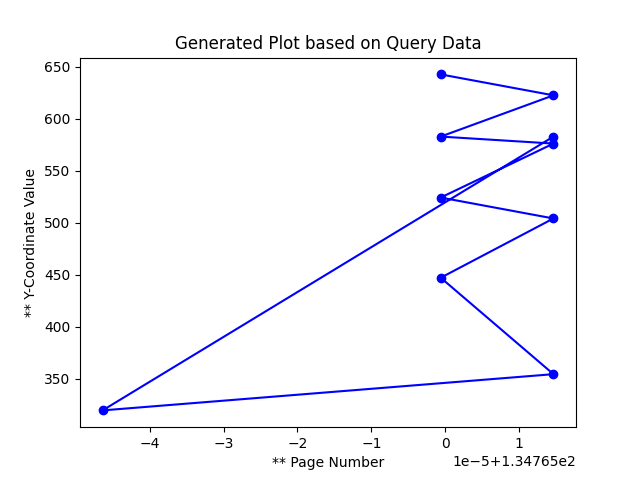
\includegraphics[width=0.9\linewidth]{plot_image.png}%
\caption{** Distribution of CNN{-}related text blocks across different page numbers, illustrating the varying y{-}coordinate values of these blocks within the research document.}%
\end{figure}

%
\end{document}